\documentclass[15pt,a5paper,reqno]{article}
\usepackage{hyperref}
\usepackage[warn]{mathtext}
\usepackage[utf8]{inputenc}
\usepackage[T2A]{fontenc}
\usepackage[russian]{babel}
\usepackage{amssymb, amsmath, multicol}
\usepackage{graphicx}
\usepackage[shortcuts,cyremdash]{extdash}
\usepackage{wrapfig}
\usepackage{gensymb}
\usepackage{floatflt}
\usepackage{lipsum}
\usepackage{verbatim}
\usepackage{concmath}
\usepackage{euler}
\usepackage{xcolor}
\usepackage{etoolbox}
\usepackage{fancyhdr}
\usepackage{subfiles}
\usepackage{enumitem}
\usepackage{amsthm}
\usepackage{indentfirst}
\usepackage{import}
\usepackage{multirow}

\DeclareMathOperator{\sign}{sign}

\RequirePackage[ left     = 1.5cm,
  right    = 1.5cm,
  top      = 2.0cm,
  bottom   = 1.25cm,
  includefoot,
  footskip = 1.25cm ]{geometry}
\setlength    {\parskip}        { .5em plus .15em minus .08em }
%\setlength    {\parindent}      { .0em }
\renewcommand {\baselinestretch}{ 1.07 }

\fancyhf{}

\renewcommand{\footrulewidth}{ .0em }
\fancyfoot[C]{\texttt{\textemdash~\thepage~\textemdash}}

\makeatletter
\patchcmd\l@section{%
  \nobreak\hfil\nobreak
}{%
  \nobreak
  \leaders\hbox{%
    $\m@th \mkern \@dotsep mu\hbox{.}\mkern \@dotsep mu$%
  }%
  \hfill
  \nobreak
}{}{\errmessage{\noexpand\l@section could not be patched}}
\makeatother
\parindent = 1cm % отступ при красной строке⏎
\pagestyle{fancy}    
\renewcommand\qedsymbol{$\blacksquare$}

\newcommand{\when}[2]{
  \left. #1 \right|_{#2} \hspace
}
\renewcommand{\kappa}{\varkappa}
\RequirePackage{caption2}
\renewcommand\captionlabeldelim{}
\newcommand*{\hm}[1]{#1\nobreak\discretionary{}

\DeclareSymbolFont{T2Aletters}{T2A}{cmr}{m}{it}
{\hbox{$\mathsurround=0pt #1$}}{}}
% Цвета для гиперссылок
\definecolor{linkcolor}{HTML}{000000} % цвет ссылок
\definecolor{urlcolor}{HTML}{799B03} % цвет гиперссылок
 
\hypersetup{pdfstartview=FitH,  linkcolor=linkcolor,urlcolor=urlcolor, colorlinks=true}


%\setcounter{secnum[utf8x]depth}{0}

\begin{document}

% НАЧАЛО ТИТУЛЬНОГО ЛИСТА
\begin{center}
  {\small ФЕДЕРАЛЬНОЕ ГОСУДАРСТВЕННОЕ АВТОНОМНОЕ ОБРАЗОВАТЕЛЬНОЕ\\ УЧРЕЖДЕНИЕ ВЫСШЕГО ОБРАЗОВАНИЯ\\ МОСКОВСКИЙ ФИЗИКО-ТЕХНИЧЕСКИЙ ИНСТИТУТ\\ (НАЦИОНАЛЬНЫЙ ИССЛЕДОВАТЕЛЬСКИЙ УНИВЕРСИТЕТ)\\ ФИЗТЕХ-ШКОЛА РАДИОТЕХНИКИ И КОМПЬЮТЕРНЫХ ТЕХНОЛОГИЙ}\\
  \hfill \break
  \hfill \break
  \hfill \break
  \Huge{Работа 2.4.1. \\ Определение теплоты испарения жидкости}\\
\end{center}

\hfill \break
\hfill \break
\hfill \break
\hfill \break
\hfill \break
\hfill \break
\hfill \break
\hfill \break

\begin{flushright}
  \normalsize{Работу выполнил:}\\
  \normalsize{\textbf{Долгов Александр Алексеевич, группа Б01-106}}\\
\end{flushright}

\begin{center}
  \normalsize{\textbf{Долгопрудный, 2022}}
\end{center}


\thispagestyle{empty} % выключаем отображение номера для этой страницы

% КОНЕЦ ТИТУЛЬНОГО ЛИСТА

\newpage
\thispagestyle{plain}
\tableofcontents
\thispagestyle{plain}
\newpage

\section{Аннотация}

    В данной работе измеряются давление насыщенного пара и теплота испарения жидкости при различных температурах. Теплота испарения определяется с помощью уравнения Клапейрона-Клаузиуса.
	
\section{Теоретические сведения}

    \textbf{Испарение} - процесс перехода вещества из жидкого состояния в газообразное. 
    
    Испарение происходит на свободной поверхности жидкости. Покинуть поверхность способны только молекулы с достаточной для этого кинетической энергией, поэтому испарение жидкости приводит к её охлаждению. Ясно, что для предотвращения охлаждения к жидкости необходимо подводить тепло.
    
    \textbf{Молярная теплота испарения} - количество теплоты, необходимое для изотермического испарения одного моля жидкости при внешнем давлении, равном давлению её насыщенного пара.
    
    \textbf{Фаза} - макроскопическая однородная часть вещества, отделённая от остальных частей системы границей раздела так, что она может быть извлечена из системы механическим путём.
    
    В случае равновесия двух фаз справедливо уравнение Клапейрона-Клаузиуса:
    \begin{equation}\label{KK_1}
        \frac{dP}{dT} = \frac{L}{T(v_2 - v_1)},
    \end{equation}
    где $P$ - давление в системе, $L$ - температура системы, $v_{1, 2}$ - молярный объём фаз 1 и 2 соответственно, $L$ - молярная теплота фазового перехода (испарения в нашем случае). Для воды: $v_{\text{вод}} = 18\cdot 10^{-6}\ \frac{\text{м}^3}{\text{моль}}$, для пара: $v_{\text{пар}} = 31\cdot 10^{-6}\ \frac{\text{м}^3}{\text{моль}}$. Из этого следует, что уравнение \eqref{KK_1} можно записать в виде:
    \begin{equation}\label{KK_2}
        \frac{dP}{dT} = \frac{L}{T\cdot v_{\text{пар}}}
    \end{equation}
    Запишем уравнение Ван-дер-Ваальса для водяного пара:
    \begin{equation}\label{vdv}
        (P + \frac{a}{v^2})(v - b) = RT
    \end{equation}
    Для водяного пара: $a = 0,4\ \frac{\text{Па}\cdot\text{м}^6}{\text{моль}^2}$, $b = 26\cdot 10^{-6}\ \frac{\text{м}^3}{\text{моль}}$. $b \ll v$, поэтому $v - b\approx v$. Слагаемым $\frac{a}{v^2}$ также можно пренебречь по сравнению с P, так как измерения проводятся при давлении ниже атмосферного. Таким образом, уравнение \eqref{vdv} переходит в уравнение состояния идеального газа:
    \begin{equation}\label{ideal}
        Pv = RT
    \end{equation}
    Подставим \eqref{ideal} в \eqref{KK_2}:
    \[\frac{dP}{dT} = \frac{PL}{RT^2} \Rightarrow L = R\frac{dP / P}{dT / T^2}\]
    \begin{equation}\label{final}
        L = -R\frac{d(\ln{P})}{d(1/T)}
    \end{equation}
    
\section{Методика измерений}

    Молярная теплота испарения определяется по формуле \eqref{final}. При этом температура жидкости измеряется термометром, давление - манометром. Производные $\frac{d(\ln{P})}{d(1/T)}$ определяются графически как угловые коэффициенты касательной к кривой, построенной в координатах, где по оси абсцисс отложена величина $\ln{P}$, а по оси ординат - величина $\frac{1}{T}$.
    
\section{Экспериментальная установка}

    Схема экспериментальной установки приведена на рисунке 1. Установка включает в себя термостат A, экспериментальный прибор B и отсчётный микроскоп С.
    
    Экспериментальный прибор B представляет собой ёмкость 12, заполненную водой. В неё погружен запаянный прибор 13 с исследуемой жидкостью 14. Перед заполнением исследуемой жидкостью воздух из прибора 13 был удалён, так что над жидкостью находится только её насыщенный пар.
    
    \begin{wrapfigure}{r}{0.6\textwidth}
        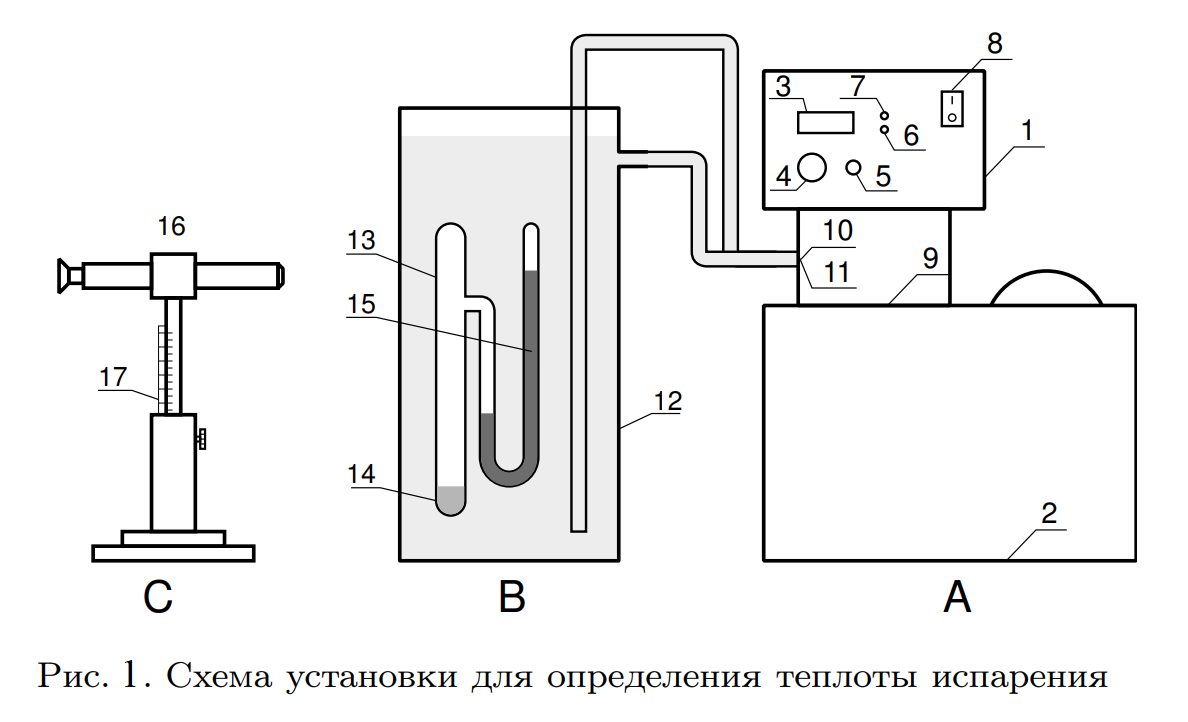
\includegraphics[width = 0.6\textwidth]{Рисунок 1.png}
    \end{wrapfigure}
    Давление пара определяется по ртутному манометру 15, соединённому с ёмкостью 13. Численная величина давления измеряется по разности показаний отсчётного микроскопа 16, настраиваемого последовательно на нижний и верхний уровни столбика ртути манометра. Показания микроскопа снимаются по шкале 17.
    
    Экспериментальная установка обладает тем недостатком, что термометр измеряет температуру термостата, а не исследуемой жидкости. Эти температуры можно считать равными, если нагревание происходит достаточно медленно (квазистатически).
    
\section{Приборы и инструментальные погрешности}

    Погрешность измерение температуры считаем равной $\sigma_t = 0.5\text{ К}$, поскольку температура флуктуировала в таких пределах в ходе практически каждого измерения (младший разряд шкалы термометра - десятые доли градуса).
    
    Давление находилось косвенно из измерений высоты ртутного столба. Давление в паскалях можно получить по формуле:
    \[P_{\text{Па}} = 13600 \cdot 9,8 \cdot h_{\text{мм}},\]
    где $P_{\text{Па}}$ - давление в паскалях, $13600$ - плотность ртути (ею заполнен манометр) в $\frac{\text{кг}}{\text{м}^3}$, $9,8$ - ускорение свободного падения вблизи поверхности Земли в $\frac{\text{Н}}{\text{кг}}$, $h_{\text{мм}}$ - высота ртутного столба в миллиметрах.
    
    Погрешностью измерения величины $h_{\text{мм}}$ считаем половину цены деления микроскопа, то есть $\sigma_{h} = 0,5\text{ мм}$. Таким образом, погрешность вычисления давления можно найти по формуле:
    \[\sigma_{P} = 13600 \cdot 9,8 \cdot \sigma_{h}\]
    
\section{Обработка полученных результатов}

    Было проведено 2 серии экспериментов по измерению зависимости давления насыщенного водяного пара от температуры. В первой серии температура термостата постепенно увеличивалась, во второй - уменьшалась. Результаты измерений приведены в таблицах 1 (нагревание) и 2 (охлаждение). По этим данным построены графики в координатах $P(T)$ (график 1: нагревание, график 3: охлаждение) и $\ln{P}(1/T)$ (график 2: нагревание, график 4: охлаждение). На каждом из графиков проведены аппроксимирующие прямые согласно методу наименьших квадратов. Обозначим коэффициент наклона прямой на $i$-м графике через $k_i$, тогда:
    \[k_1 = (209 \pm 7)\ \frac{\text{Па}}{\text{К}}\]
    \[k_2 = (-5,93 \pm 0.05)\cdot 10^3\ \text{К}\]
    \[k_3 = (231 \pm 6)\ \frac{\text{Па}}{\text{К}}\]
    \[k_4 = (-6.3 \pm 0.2)\cdot 10^3\ \text{К}\]
    Теперь получим молярные теплоты парообразования по графикам 2 и 4. Из \eqref{final} получаем:
    \[L_{2,4} = -k_{2,4}R;\ \ \ \sigma_L = \sigma_k R\]
    Поэтому:
    \[L_2 = (49300 \pm 400)\ \frac{\text{Дж}}{\text{моль}\cdot\text{К}}\]
    \[L_4 = (52400 \pm 1700)\ \frac{\text{Дж}}{\text{моль}\cdot\text{К}}\]
    
    Для сравнения двух серий также построен график 5 в координатах $P(T)$, содержащий лишь экспериментальные точки обеих серий.
    
\section{Вывод}

    В ходе работы были получены два значения молярной теплоты парообразования воды. Оба результата не совпадают с табличным значением, которое равно $L = 40662\ \frac{\text{Дж}}{\text{моль}\cdot\text{К}}$. Объяснить такое несоответствие можно неточностью измерения давления, так как оно измерялось человеком, а не электронным прибором как температура. Тем не менее результат, найденный из данных, соответствующих нагреванию воды, оказался более точным как в смысле относительной погрешности, так и в смысле близости к истинному результату.

\newpage
\section{Приложения}

    \subsection{Таблица 1. Нагревание}
    \begin{tabular}{|c|c|c|c|c|c|}
        \hline
        T, К  &  $\sigma_T$, К        & h, мм & $\sigma_h$, мм         & P, Па & $\sigma_P$, мм      \\ \hline
        296,0 & \multirow{12}{*}{0,5} & 15,8  & \multirow{12}{*}{0,05} & 2106  & \multirow{12}{*}{7} \\ 
        297,2 &                       & 17,5  &                        & 2332  &                     \\ 
        298,0 &                       & 18,2  &                        & 2426  &                     \\ 
        299,1 &                       & 19,4  &                        & 2586  &                     \\ 
        300,1 &                       & 20,8  &                        & 2772  &                     \\ 
        301,1 &                       & 22,3  &                        & 2972  &                     \\ 
        302,9 &                       & 25,2  &                        & 3359  &                     \\ 
        304,0 &                       & 26,8  &                        & 3572  &                     \\         
        305,0 &                       & 28,4  &                        & 3785  &                     \\         
        306,0 &                       & 30,6  &                        & 4078  &                     \\        
        307,0 &                       & 32,7  &                        & 4358  &                     \\       
        308,0 &                       & 34,9  &                        & 4651  &                     \\ \hline
    \end{tabular}
    
    \subsection{Таблица . Охлаждение}
    \begin{tabular}{|c|c|c|c|c|c|}
        \hline
        T, К  &  $\sigma_T$, К        & h, мм & $\sigma_h$, мм         & P, Па & $\sigma_P$, мм      \\ \hline
        307,0 & \multirow{12}{*}{0,5} & 34,5  & \multirow{12}{*}{0,05} & 4598  & \multirow{12}{*}{7} \\ 
        306,0 &                       & 33,5  &                        & 4465  &                     \\ 
        305,0 &                       & 32,7  &                        & 4358  &                     \\ 
        304,0 &                       & 30,5  &                        & 4065  &                     \\ 
        303,0 &                       & 28,8  &                        & 3838  &                     \\ 
        302,0 &                       & 26,1  &                        & 3479  &                     \\ 
        301,0 &                       & 25,2  &                        & 3359  &                     \\ 
        300,0 &                       & 22,7  &                        & 3025  &                     \\         
        299,0 &                       & 21,4  &                        & 2852  &                     \\         
        298,0 &                       & 19,5  &                        & 2599  &                     \\        
        297,0 &                       & 17,9  &                        & 2386  &                     \\       
        296,0 &                       & 16,5  &                        & 2199  &                     \\ \hline
    \end{tabular}

    \newpage
    \subsection{График 1. P(T) при нагревании}
    \begin{center}
        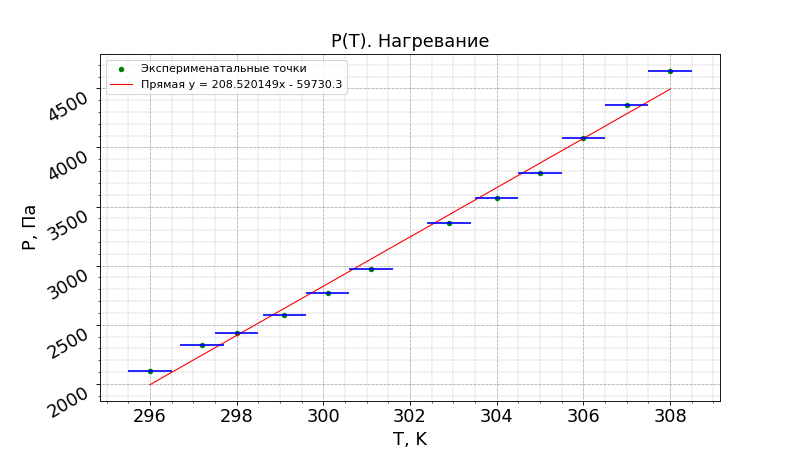
\includegraphics[width = \textwidth]{График 1.png}
    \end{center}
    
    \subsection{График 2. ln(P) (1/T) при нагревании}
    \begin{center}
        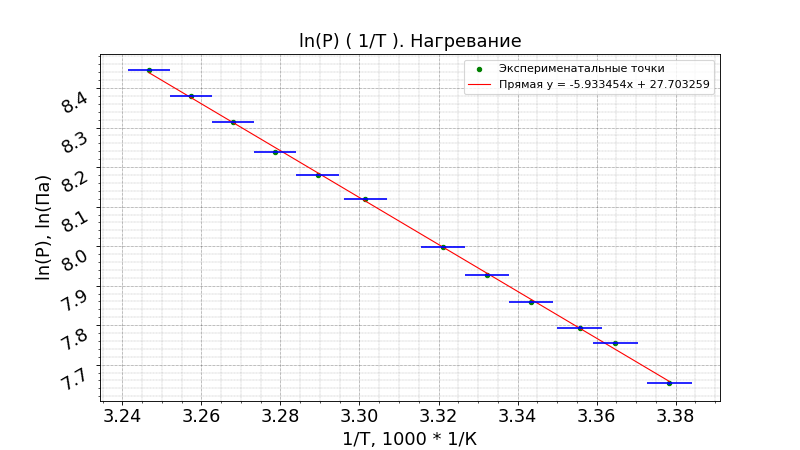
\includegraphics[width = \textwidth]{График 2.png}
    \end{center}
    
    \subsection{График 3. P(T) при охлаждении}
    \begin{center}
        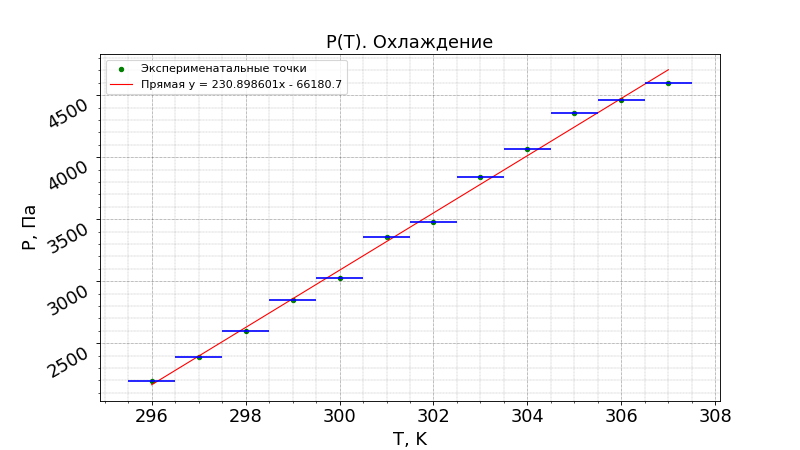
\includegraphics[width = \textwidth]{График 3.png}
    \end{center}
    
    \subsection{График 4. ln(P) (1/T) при охлаждении}
    \begin{center}
        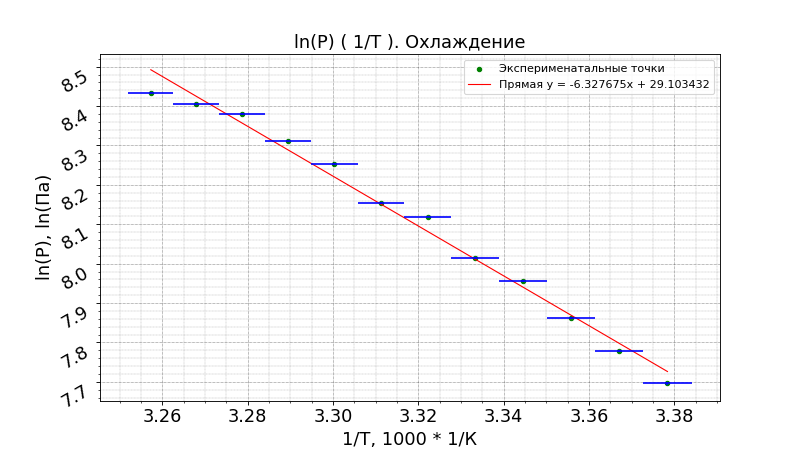
\includegraphics[width = \textwidth]{График 4.png}
    \end{center}
    
    \subsection{График 5. Нагревание и охлаждение}
    \begin{center}
        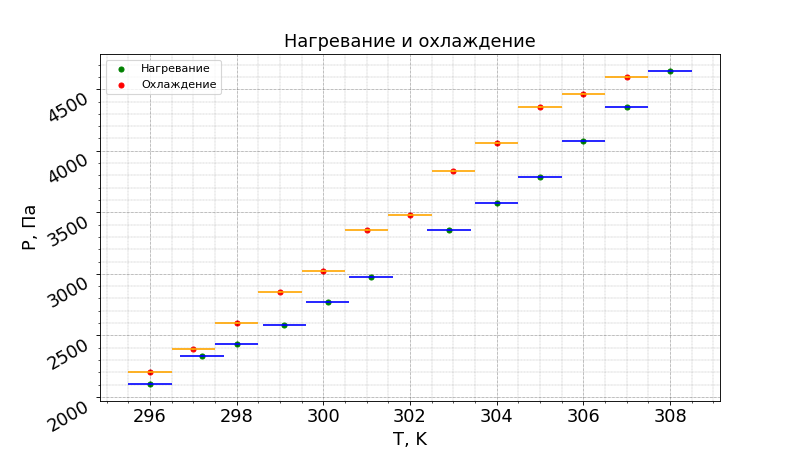
\includegraphics[width = \textwidth]{График 5.png}
    \end{center}

\end{document}